
%%% Local Variables:
%%% mode: latex
%%% TeX-master: t
%%% End:
\documentclass[mathserif]{beamer}
\usepackage{tikz}
\usepackage[T1]{fontenc}
\usepackage{xeCJK}
\usetikzlibrary{arrows,decorations.pathmorphing,backgrounds,positioning,fit,petri}

\usetheme{Boadilla}
\usecolortheme{seagull}

\usepackage[listings]{tcolorbox}
\newtcblisting{source}{
    listing only,
    listing options={style=tcblatex,moredelim={**[is][\color{red}]{@}{@}}}
}

\title{tikz实例2}

\begin{document}
\begin{frame}
  \maketitle
\end{frame}

\begin{frame}[fragile]{node}{}
\begin{tikzpicture}
\path ( 0,2) node [shape=circle,draw] {}
      ( 0,1) node [shape=circle,draw] {}
      ( 0,0) node [shape=circle,draw] {}
      ( 1,1) node [shape=rectangle,draw] {}
      (-1,1) node [shape=rectangle,draw] {};
\end{tikzpicture}
\end{frame}

\begin{frame}[fragile]\frametitle{node at}
\begin{tikzpicture}
\path node at ( 0,2) [shape=circle,draw] {}
      node at ( 0,1) [shape=circle,draw] {}
      node at ( 0,0) [shape=circle,draw] {}
      node at ( 1,1) [shape=rectangle,draw] {}
      node at (-1,1) [shape=rectangle,draw] {};
\end{tikzpicture}
\hspace{20pt}
\begin{tikzpicture}
\node at ( 0,2) [circle,draw] {};
\node at ( 0,1) [circle,draw] {};
\node at ( 0,0) [circle,draw] {};
\node at ( 1,1) [rectangle,draw] {};
\node at (-1,1) [rectangle,draw] {};
\end{tikzpicture}  
\end{frame}

\begin{frame}[fragile]\frametitle{node样式}
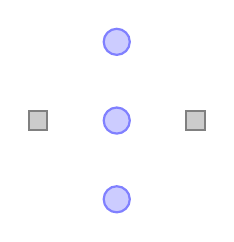
\begin{tikzpicture}[thick]
\node at ( 0,2) [circle,draw=blue!50,fill=blue!20] {};
\node at ( 0,1) [circle,draw=blue!50,fill=blue!20] {};
\node at ( 0,0) [circle,draw=blue!50,fill=blue!20] {};
\node at ( 1,1) [rectangle,draw=black!50,fill=black!20] {};
\node at (-1,1) [rectangle,draw=black!50,fill=black!20] {};
\end{tikzpicture}
\hspace{20pt}
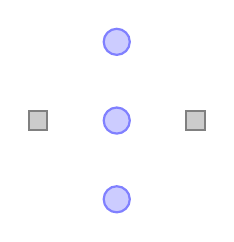
\begin{tikzpicture}
[place/.style={circle,draw=blue!50,fill=blue!20,thick},
transition/.style={rectangle,draw=black!50,fill=black!20,thick}]
\node at ( 0,2) [place] {};
\node at ( 0,1) [place] {};
\node at ( 0,0) [place] {};
\node at ( 1,1) [transition] {};
\node at (-1,1) [transition] {};
\end{tikzpicture}

\begin{frame}[fragile]\frametitle{node尺寸}
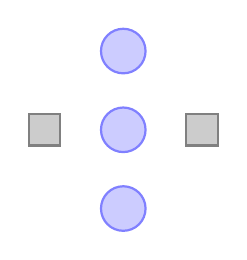
\begin{tikzpicture}
[inner sep=2mm,
place/.style={circle,draw=blue!50,fill=blue!20,thick},
transition/.style={rectangle,draw=black!50,fill=black!20,thick}]
\node at ( 0,2) [place] {};
\node at ( 0,1) [place] {};
\node at ( 0,0) [place] {};
\node at ( 1,1) [transition] {};
\node at (-1,1) [transition] {};
\end{tikzpicture}
\hspace{20pt}
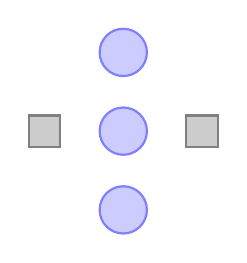
\begin{tikzpicture}
[place/.style={circle,draw=blue!50,fill=blue!20,thick,
inner sep=0pt,minimum size=6mm},
transition/.style={rectangle,draw=black!50,fill=black!20,thick,
inner sep=0pt,minimum size=4mm}]
\node at ( 0,2) [place] {};
\node at ( 0,1) [place] {};
\node at ( 0,0) [place] {};
\node at ( 1,1) [transition] {};
\node at (-1,1) [transition] {};
\end{tikzpicture}  
\end{frame}  
\end{frame}
\end{document}
